\chapter{Data Extraction and Preprocessing} 
\label{Chapter3}

This chapter details the data sources used to train the various loan default prediction models developed throughout this project, the various data extraction techniques used to extract the alternative features within the training sets, and the pre-processing and feature engineering techniques deployed before the modelling phase.   
%---------------------------------------------------------------------------------------
%	SECTION 1
%---------------------------------------------------------------------------------------

\section{Data Used}

\subsection{Providers}

The models in this project are trained using data from two main sources \\

The first data provider is a Nigerian micro-finance institution that has disbursed loans to more than 250,000 consumers. The institution is an application (app) based lender and currently only provides credit to android users. The institution, with its customers' consent, gains access to the data on customers' devices. This data includes SMS data, contact data and location data. On top of the alternative data collected, sociodemographic data is collected via customer input on the institution's mobile app. \\

The second source of data for this project was the Nigerian credit bureaus CRC, CRS and XDS. It is mandatory for credit providing institutions in Nigeria to submit their customers' credit performance data to these credit bureaus.

\subsection{Personal Data}

It is key to note that no personal data - data that relates to an individual or could be used to identify a living individual - was made publicly available, used within the creation of features, or used to train the models developed throughout this project. 

\subsection{Dataset}

A final dataset was created for first time loan customers of the micro-finance institution that had existing credit bureau data prior to their first loan application. The customers required existing credit data as it was needed in order to compare the performance of first time credit credit scoring models that use only alternative data or alternative data in conjunction with sociodemographic data, against first time credit scoring models that make use of existing credit data. The final dataset consisted of 62,935 customers/loans. \newpage

\subsection{Data Categories}

Three major data categories can be drawn from the data sources. These categories are sociodemographic data, credit bureau data and alternative data. The main aim of this thesis is to assess how alternative data can augment traditional credit scoring data. To complete this aim various combinations of these data categories are used to develop various credit scoring models. These models are a logistic regression model, a random forest model, an extreme gradient boosted model, and a neural network. The statistical performance of the models is assessed in order to test whether using the various data categories resulted in a significant difference in model performance. 

\subsection{Variables Used}

Table \ref{table:variables}, which can be found in the appendix attached to this report, displays all variables used to train the loan default prediction models. All sociodemographic variables used are stated by the loan applicants. The variables derived from app and SMS data are scraped from the loan applicants' devices. The variables relating to each applicant's credit history are provided by the Nigerian credit bureaus. \\

The following figures display the traits of specific independent variables used in the models of this project. The figures show the relationship between the independent variables and the dependent variable (whether a loanee repaid their loan).  

\subsubsection{Repayment Breakdown}

Figure \ref{fig:defaulted} displays the breakdown of the first time loans used to train this project's models. It can be seen from the figure that 49,596 of the total 62,935 loans considered for this project were repaid. That means that the default rate of loans considered was 21.19\%. This is a high default rate when compared to default rates in Western countries, but in underdeveloped countries - like Nigeria - this aligns with industry standard \parencite{Default}.

\vspace{10 pt}

\begin{figure}[!htb]
\centering
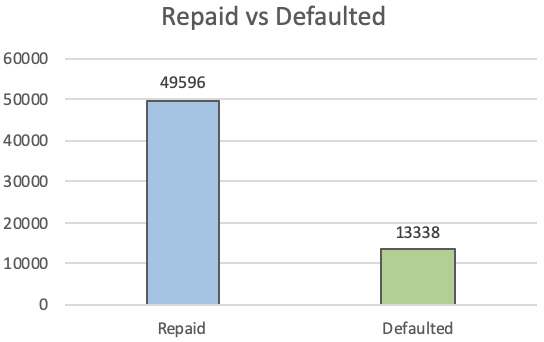
\includegraphics[width=0.45\textwidth]{images/payments.png}
\caption{Repaid vs Defaulted}
\label{fig:defaulted}
\end{figure}

\subsubsection{Age of Loanees}

Figures \ref{fig:age_paid} and \ref{fig:age_defaulted} display a comparison between the age of the clients that repaid their loan and the age of clients that defaulted on their loan. It can be seen from the figures that the percentage of clients 30 or younger is considerably higher for clients that defaulted compared to clients that repaid. Figure \ref{fig:age_defaulted} is skewed to the right when compared to Figure \ref{fig:age_paid}, which means that on the whole the sample of clients that defaulted is younger than the sample of clients that repaid.   

\vspace{10 pt}

\begin{figure}[!htb]
\centering
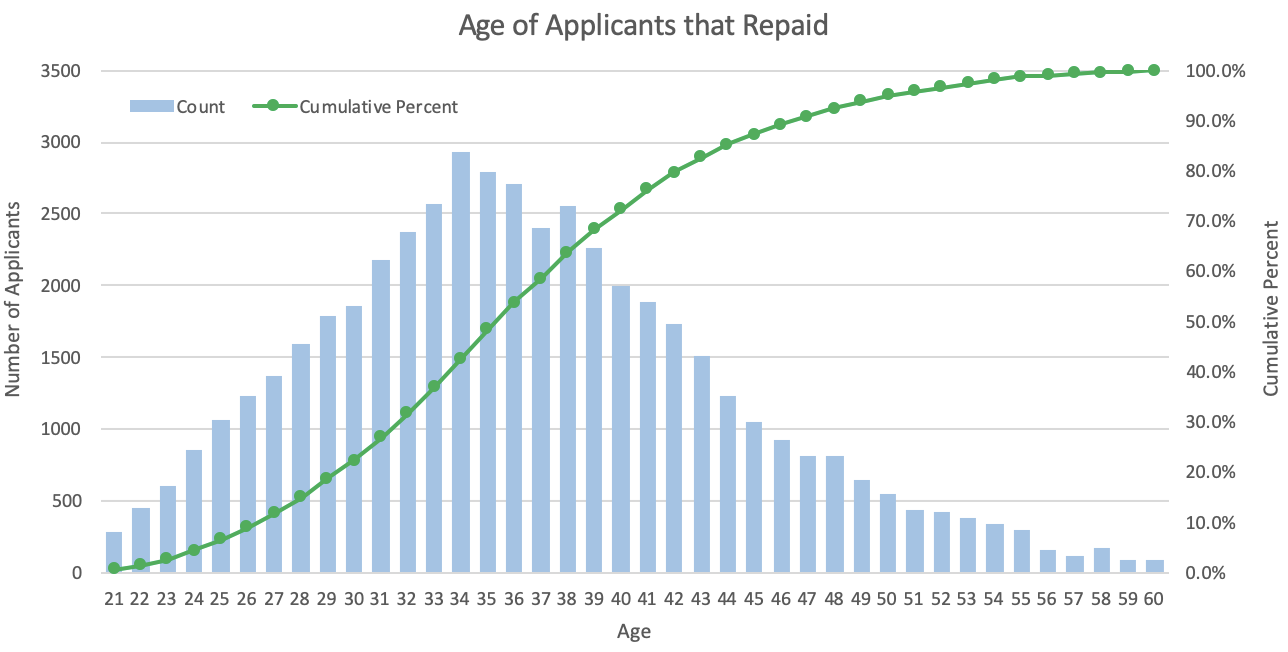
\includegraphics[width=0.65\textwidth]{images/repaid_age.png}
\caption{Age of Clients that Repaid}
\label{fig:age_paid}
\end{figure}

\vspace{10 pt}

\begin{figure}[!htb]
\centering
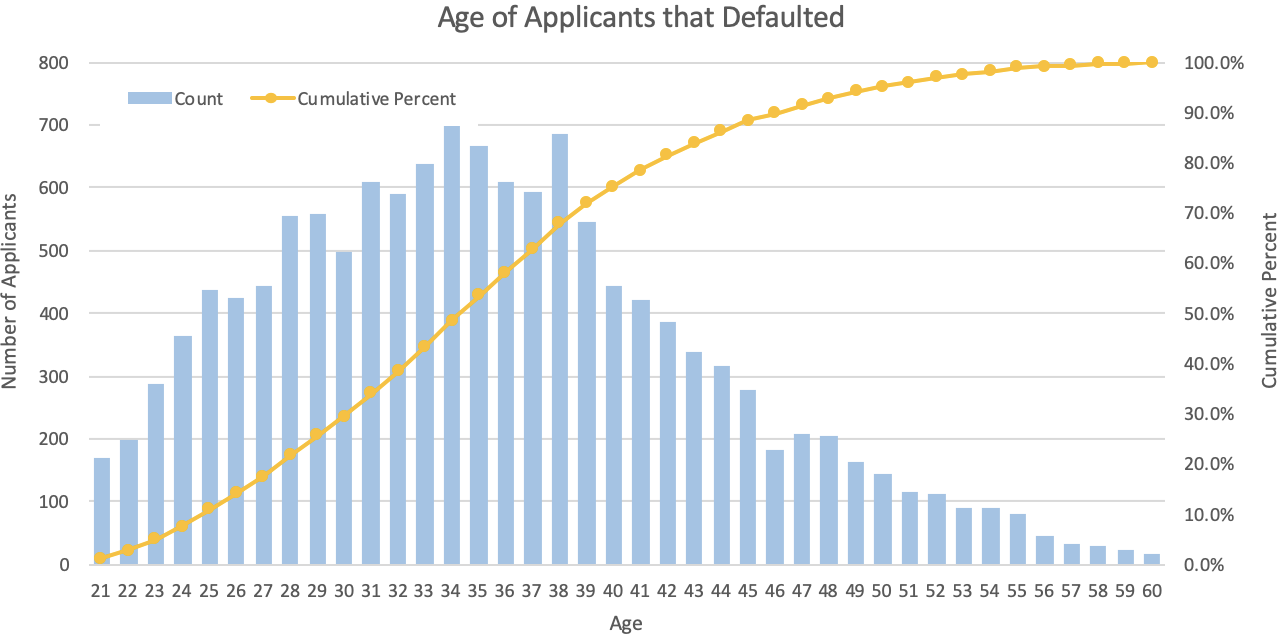
\includegraphics[width=0.65\textwidth]{images/defaulted_age.png}
\caption{Age of Clients that Defaulted}
\label{fig:age_defaulted}
\end{figure}

\vspace{10 pt}

\subsubsection{Income of Loanees}

Figures \ref{fig:income_paid} and \ref{fig:income_defaulted} display a comparison between the incomes of the clients that repaid their loan and the incomes of clients that defaulted on their loan. The a larger percentage of clients that defaulted on their loan have an income of 700,000 Naira or less than clients that repaid their loan.   

\vspace{10 pt}

\begin{figure}[!htb]
\centering
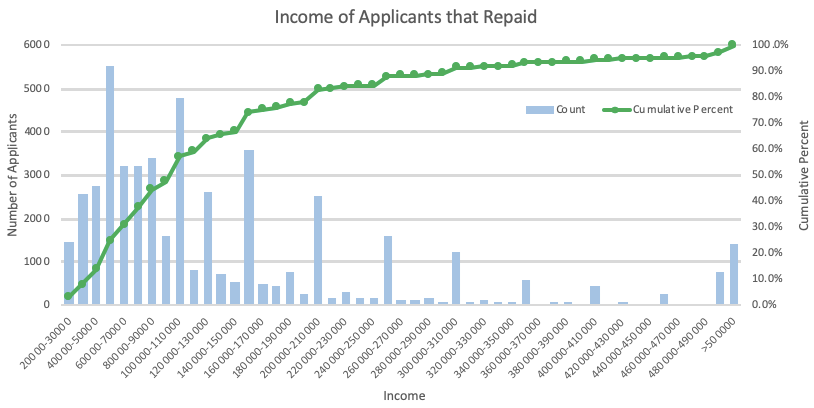
\includegraphics[width=0.75\textwidth]{images/repaid_income.png}
\caption{Income of Clients that Repaid}
\label{fig:income_paid}
\end{figure}

\vspace{10 pt}

\begin{figure}[!htb]
\centering
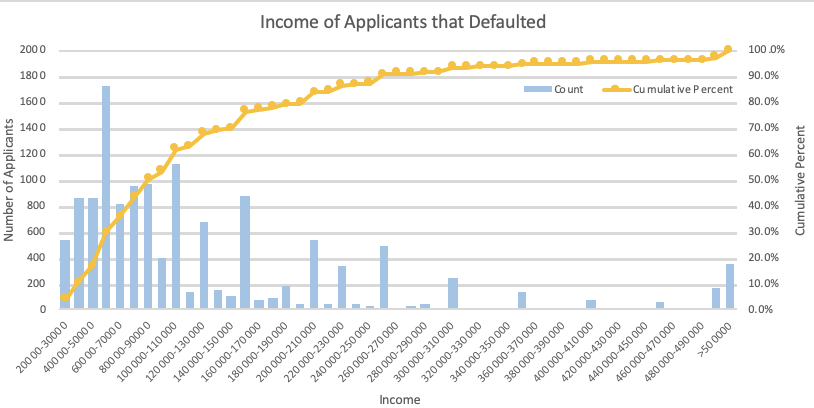
\includegraphics[width=0.75\textwidth]{images/defaulted_income.png}
\caption{Income of Clients that Defaulted}
\label{fig:income_defaulted}
\end{figure}

\vspace{10 pt}

\subsubsection{Employment Status and Gender}

Figure \ref{fig:employment} displays the various employment statuses of the considered clients. The figure further displays the number of male and female clients contained in employment status and their default rates for their loans. 

\vspace{10 pt}

\begin{figure}[!htb]
\centering
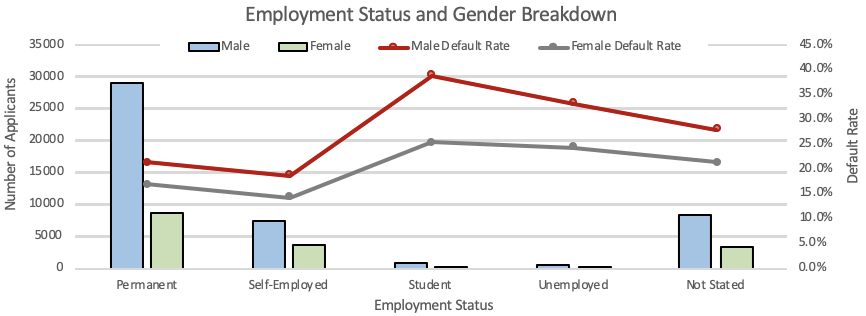
\includegraphics[width=0.9\textwidth]{images/employment.png}
\caption{Employment Status and Gender of Clients}
\label{fig:employment}
\end{figure}

\vspace{10 pt}

Figure \ref{fig:employment} shows that the majority of loanees claimed that they are permanently employed and that there were more male loanees contained in the sample than female loanees. The figure further shows that generally students and unemployed loanees are more likely to default. Finally the figure displays that female loanees generally perform better than male loanees.  

\subsubsection{Credit Bureau Accounts and Gender}


Figure \ref{fig:cred} displays the number of female and male clients that have a specific number of registered accounts with the Nigerian credit bureaus. The figure also displays the default rate by the number of registered accounts. Figure \ref{fig:cred} - like Figure \ref{fig:employment} - displays that there are more male loanees in the sample than female and that female loanees tend to repay better than male loanees. Figure \ref{fig:cred} further displays that the most clients only had 1 account registered with the credit bureaus and that in general the more accounts a client has registered with the credit bureaus, the more likely they are to repay their loan.  

\vspace{10 pt}

\begin{figure}[!htb]
\centering
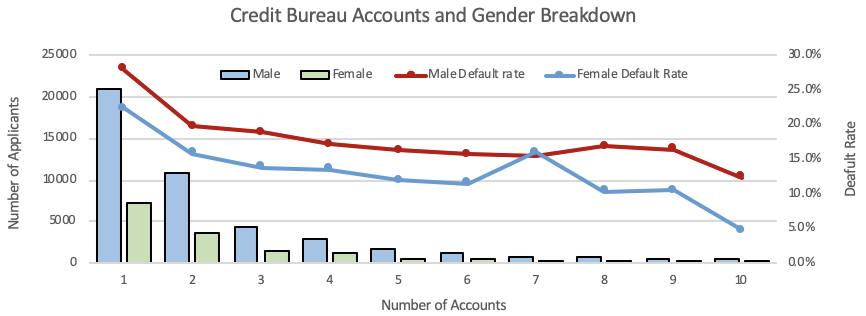
\includegraphics[width=0.9\textwidth]{images/credit_bur.png}
\caption{Number of Credit Bureau Accounts and Gender of Clients}
\label{fig:cred}
\end{figure}

\vspace{10 pt}

The sources of data and the data itself used throughout the project has now been described. Section 3.2 details how the data is gathered and the processes used to generate the variables used in the models of this project.   

%---------------------------------------------------------------------------------------
%	SECTION 2
%---------------------------------------------------------------------------------------

\section{Data Extraction and Feature Engineering}

This section details the data extractions and feature engineering techniques used throughout this project. The processes to gather the sociodemographic and credit bureau data require are simpler than those used to gather the alternative data.

\subsection{Sociodemographic and Credit Bureau Data}

The more traditional credit scoring features, developed from sociodemographic and credit bureau data attached to each first-time borrower, were created and extracted using SQL (Structured Query Language). The data was extracted from the company's relational database. \\

The query was written in a manner that ensured that no data leakage would occur when the credit scoring models were being trained. This means that only data that would be known at the point in time when a particular client applied for their loan could be used to develop features. The only case where data was used that would not be known at the point in time of application was repayment data, as this was used to develop the default (whether the client repaid their loan or not) target variable. \\

The overall query used to extract the sociodemographic and credit bureau data for each loan was a collection of sub-queries joined on a unique key attached to each loan. The query used to extract the credit bureau required an aggregation in order to generate features that represented the total number of loans each client had prior to their loan application with the micro-finance institution used in this study. The credit bureau features used in the modelling process and their definitions can be found in the appendix of this paper.

\subsection{Alternative Data}

The three main sources of alternative data used to develop features are the app-based, SMS, and device data stored on each customers' cellphone. The data is extracted from one of the micro-finance institution's  databases using PyMongo, a Python package that allows a user to query data from a Mongo database from within a Python script. \newpage

The app-based and SMS data is extracted from a different Mongo databases, however regular expressions (regex) are used to filter both data types and to develop features. Regex functions are sets of sequences of characters that define a particular search pattern. The functions are then used to identify cases of the defined pattern in strings \parencite{Regex}. \\

The device data is extracted from a separate database than the app and SMS data and an entirely different technique is used to collect the data. The technique used in this case is web scraping, which is a method of extracting data from websites \parencite{WebScraping}. 

\subsubsection{App-Based Features}

The app-based features engineered for this project are counts of particular apps present on a client's device at the point in time of their loan application. The features included a count of the financial, competing micro-finance, news, gambling and virtual private network (VPN) apps. The counts are generated by first compiling a list of all unique apps on a client's device. Then the name of each app is passed through a series of regular expression key word searches. Each expression is designed to detect a specific app type. If a particular app type search results in a match, the count associated with that search is updated. \\

The process developed to pass an app through the app extracting regular expressions and how the count features are generated throughout this process is represented in Figure \ref{fig:app_features}. The process is completed for every unique app recorded on the client's device. 


\vspace{10 pt}

\begin{figure}[!htb]
\centering
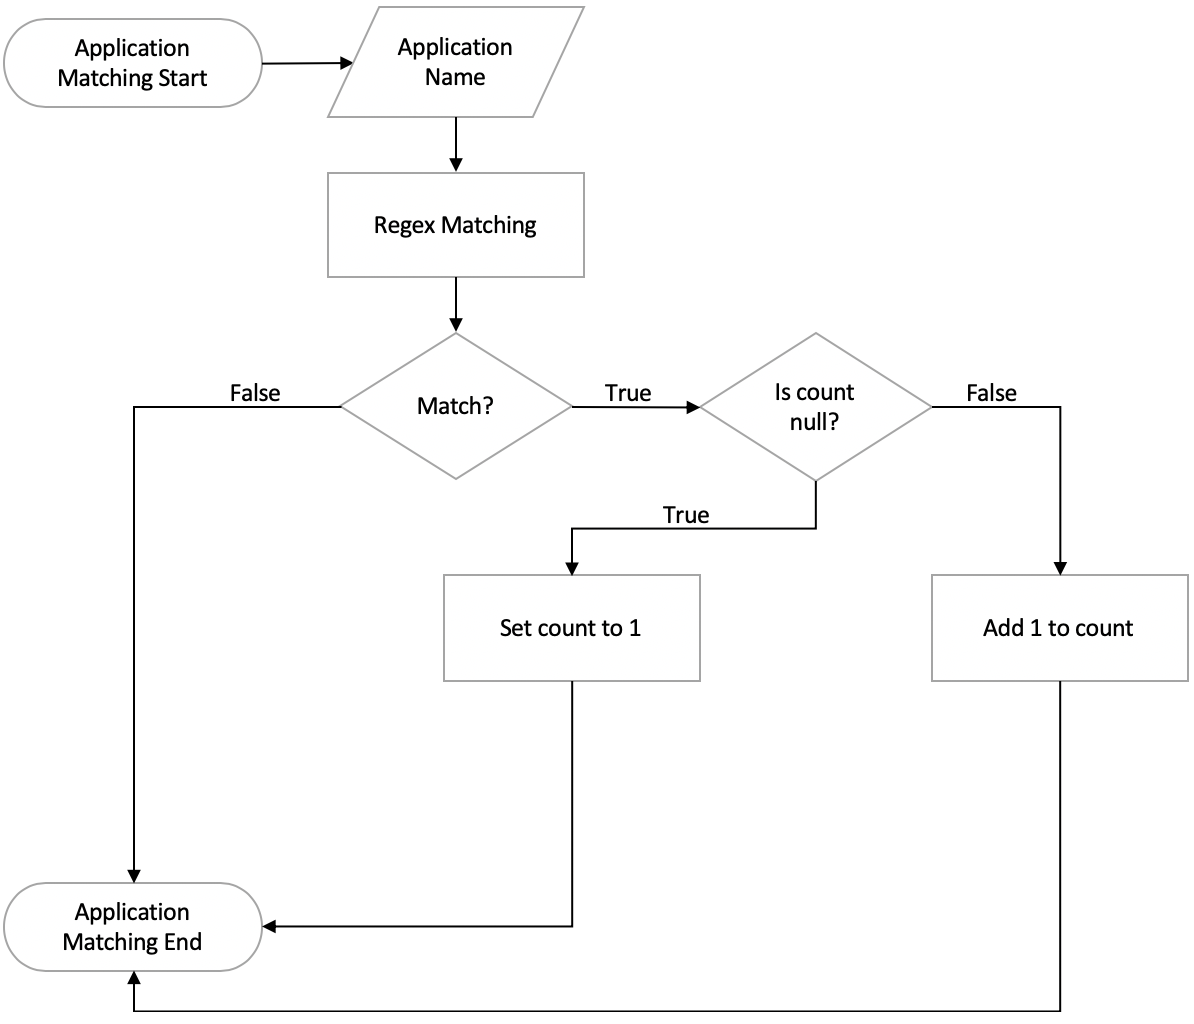
\includegraphics[width=0.9\textwidth]{images/app_feats.png}
\caption{App-Based Feature Generation}
\label{fig:app_features}
\end{figure}

\newpage

\subsubsection{SMS-Based Features}

The SMS data consists of messages received by the clients in the 90 days prior to their loan application: by nature this data is more sensitive than the other data used throughout this research. Similar to the process developed to generate the app-based features, each message received by a client is compiled into a list. Each individual message in their list is then passed through a series of regular expressions in order to generate features.  \\

In order to avoid exposing personal messages, each message was passed through two filtering regular expressions. The first expression returned only messages received from Nigerian banks, while the second ensured that only messages returned by competitor micro-finance institutions were returned. The regular expressions had a dual purpose: they prevented exposure to sensitive content and they acted as the first step in the SMS-based feature generation process. \\

If a message passes through the regular expression for banking messages it is exposed to the banking feature creation process. Typically, messages from Nigerian banks have a similar structure. They display a transaction amount, the date of the transaction, the type of transaction (credit or debit to the account), and finally the balance in the account after the transaction. Regular expressions are used to extract these features and store them as either numeric variables or lists.  \\

If a message did not pass through the first filter regular expression - searching for bank messages - it is then passed through the competitor expression. If the message passes through this expression it is then further screened by another set of regex functions. These functions search for key words in order to determine if a client had another loan with a competitor and if that loan had been repaid successfully or not. The actual loan amount is extracted using regex, as is the loan repayment (instalment amount). These amounts were appended to lists. \\

After passing every message associated to a particular client through the regex functions the lists created throughout the process are used to generate the SMS-based features for that particular client. \\

\vspace{10pt}

The banking related features generated were:

\begin{itemize}
    \item The number of unique banks that sent the client a message
    \item The minimum and maximum debit transaction, credit transactions and account balance values 
    \item The total number of debit and credit transactions 
    \item The number of times the term 'insufficient funds' is found in the client's messages
\end{itemize}

\vspace{10pt}

The process of passing an SMS through the bank related regular expressions and how the banking features are generated throughout that process is represented in Figure \ref{fig:bank_features}. The process is completed for every message received by a client within the 90-day period prior to their loan application. 

\vspace{10pt}

\begin{figure}[!htb]
\centering
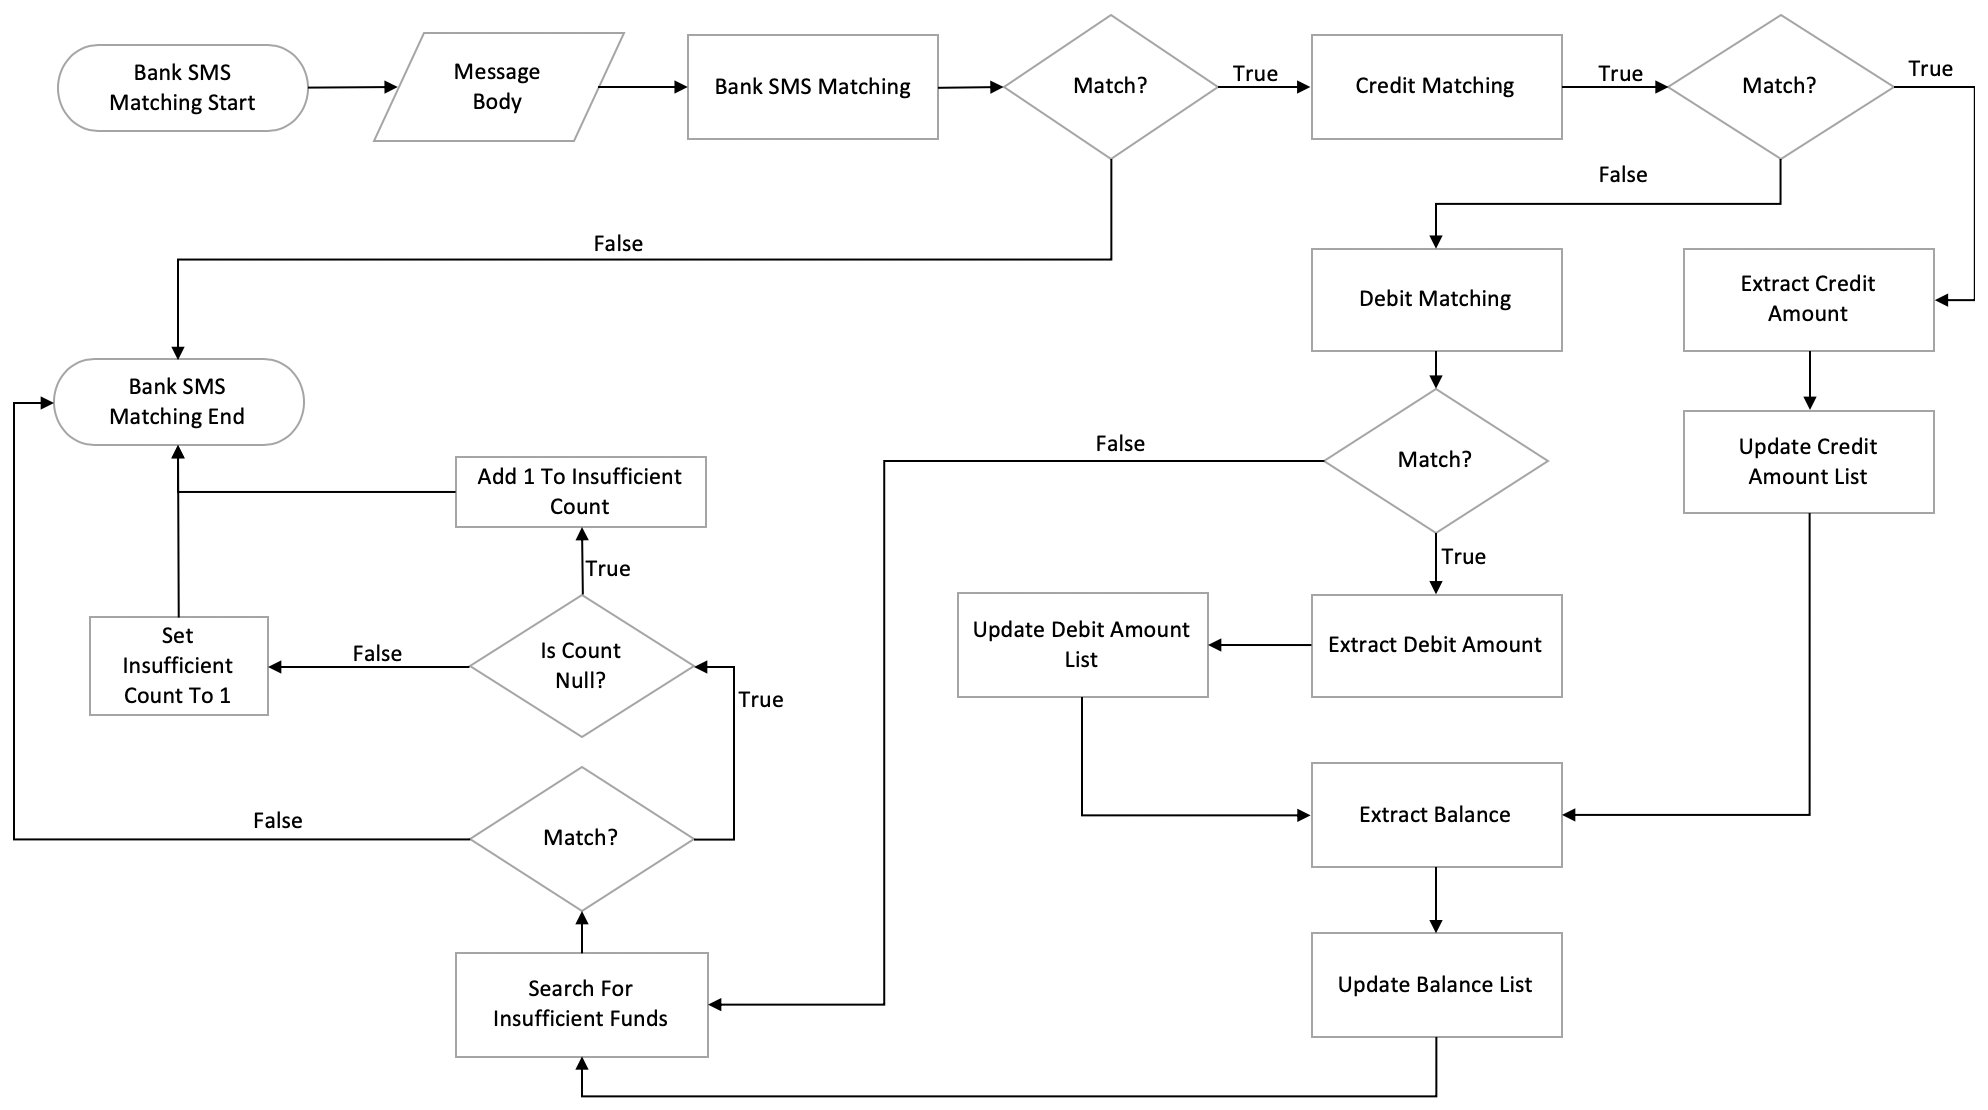
\includegraphics[width=0.95\textwidth]{images/bank_feats.png}
\caption{Bank Based Feature Generation}
\label{fig:bank_features}
\end{figure}

\vspace{10pt}

\newpage

The competitor related features generated were:

\begin{itemize}
    \item The number of competitors that sent the client a message
    \item The number of competitors that approved a loan for the client
    \item The minimum and maximum loan amount received by, successful loan repayment made by, and unsuccessful loan repayment made by the client
    \item The number of loans received by, successful loan repayments made by, and unsuccessful loan repayments made by the client
    \item The number of rejected loan applications made by the client. 
\end{itemize}

\vspace{10pt}

The process of passing an SMS through the competitor related regular expressions and how features are generated throughout that process is represented in Figure \ref{fig:comp_features}. The process was completed for every SMS message received by a client within the 90-day period prior to their application. 

\vspace{10pt}

\begin{figure}[!htb]
\centering
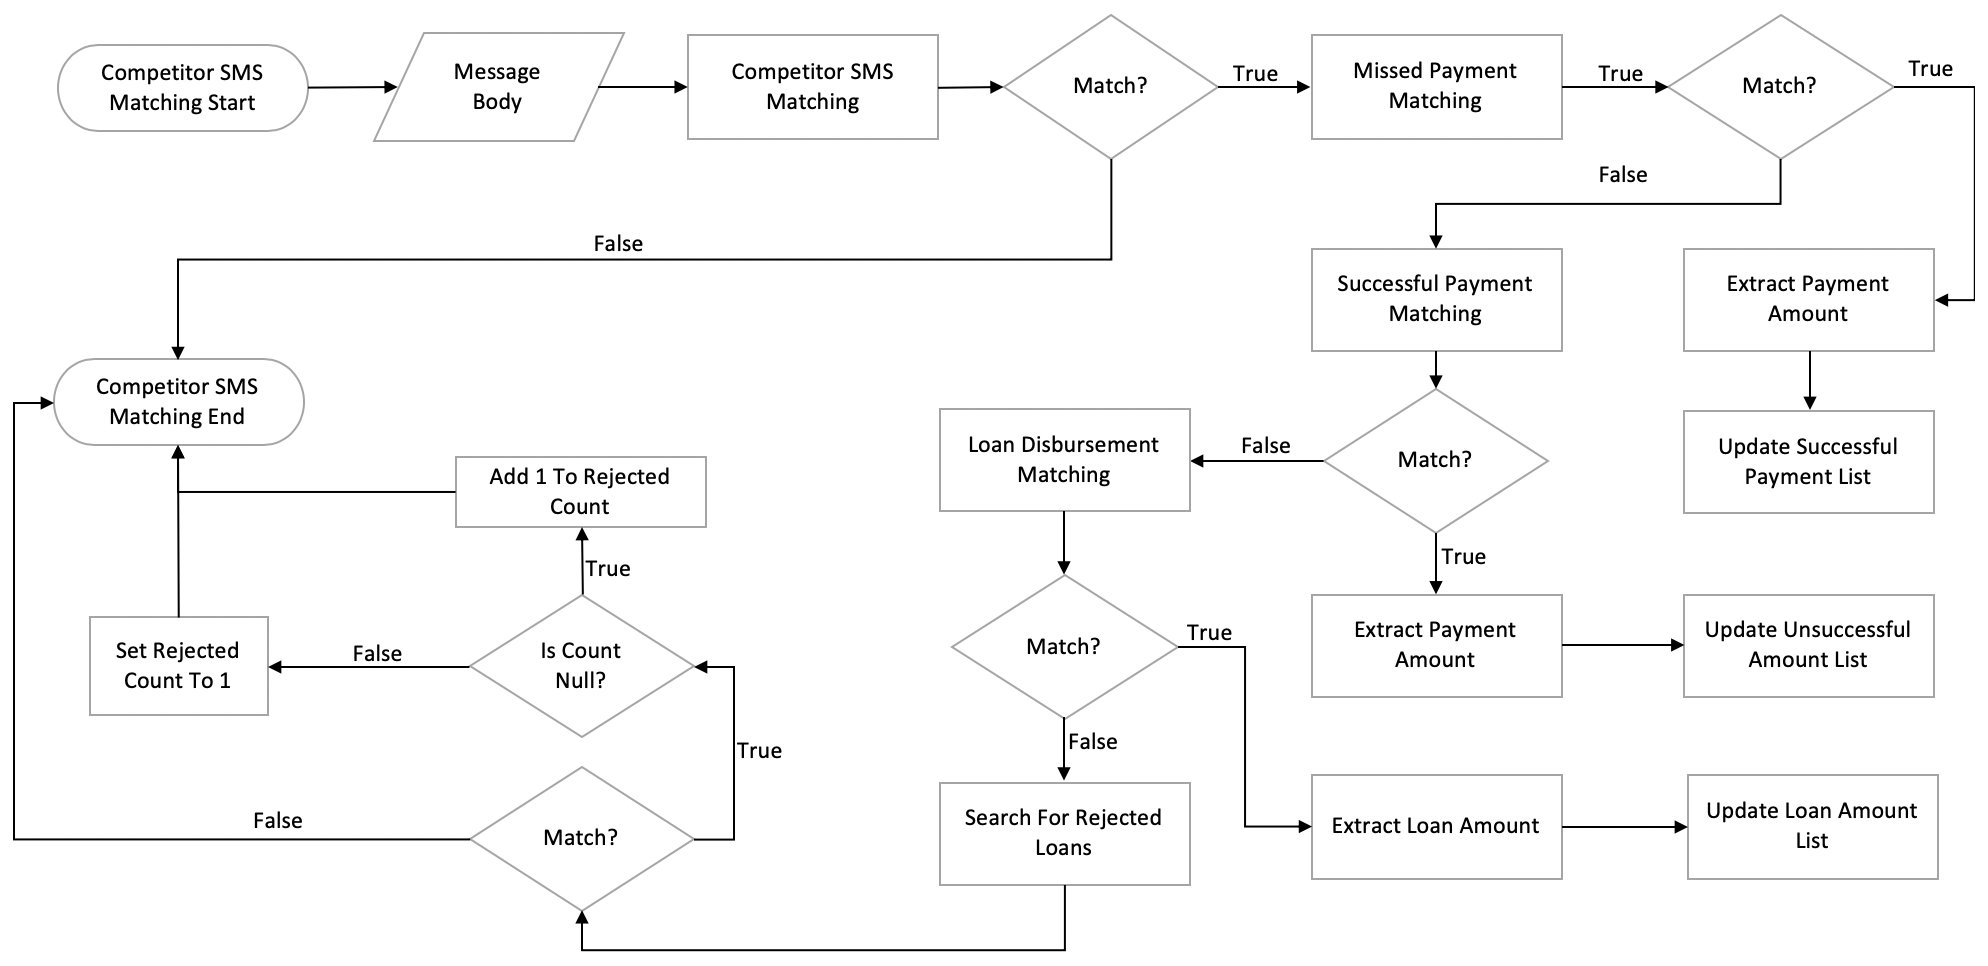
\includegraphics[width=0.95\textwidth]{images/comp_feats.png}
\caption{Competitor Based Feature Generation}
\label{fig:comp_features}
\end{figure}

\vspace{10pt}


\subsubsection{Web Scraping}

The unique Android ID attached to each customer's cellular device - used when applying for their loan - is used to ascertain the brand and model of the device as well as the device's operating system version. The brand of device and operating system are used directly as features while the brand name and device model were used in conjunction to scrape the price of the device. \\

The script written to scrape and derive the device price was written in Python and made use of the Beautiful Soup web scraping package. The price of each device was scraped from Jumia and Kara, two of the biggest Nigerian e-commerce platforms. \\

The logic used to derive a price for each customer's cellular device is shown in Figure \ref{fig:device}.

\vspace{10pt}

\begin{figure}[!htb]
\centering
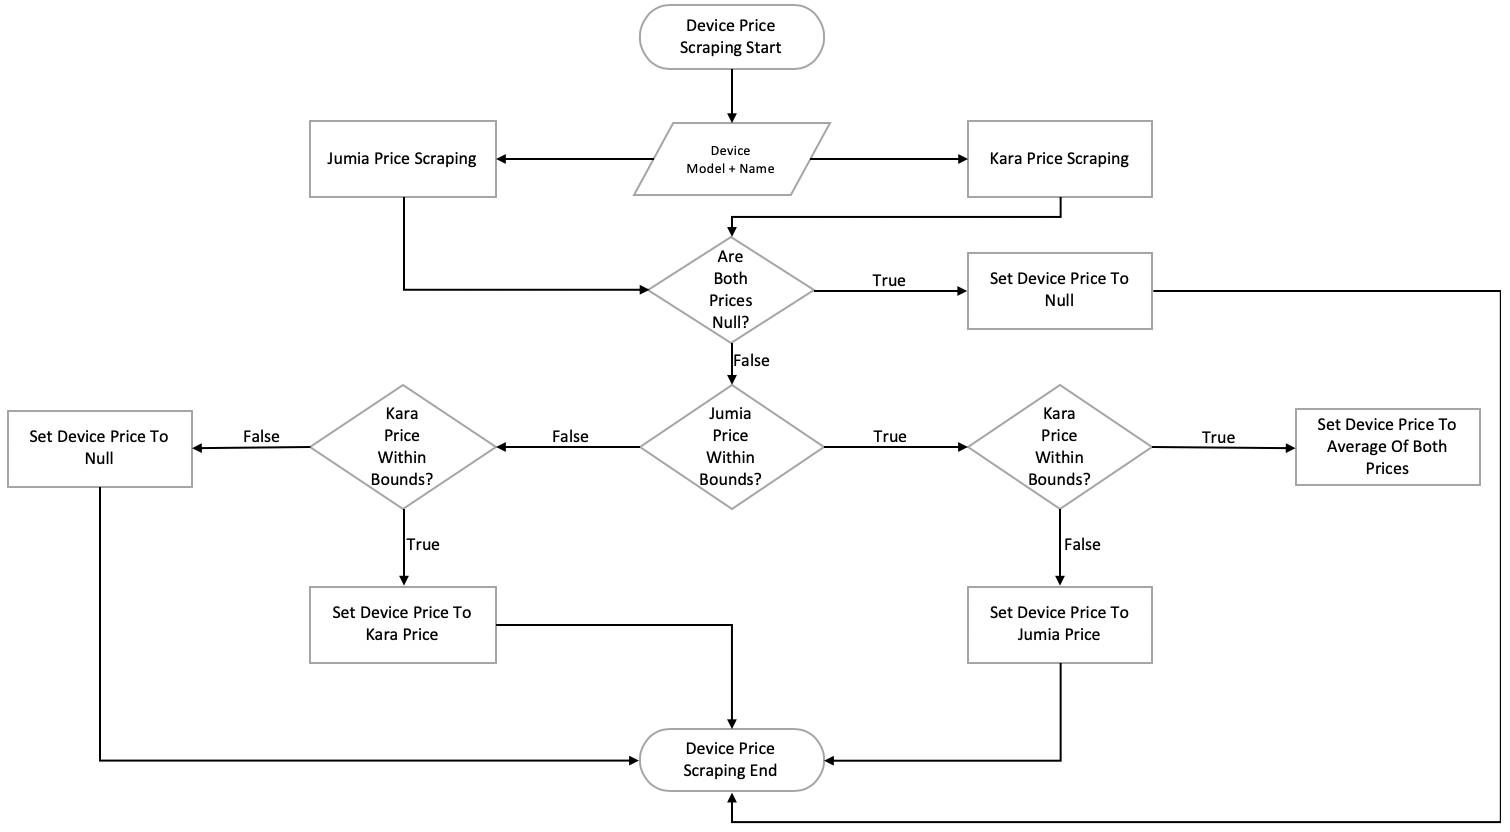
\includegraphics[width=0.95\textwidth]{images/device_price.png}
\caption{Device Price Logic}
\label{fig:device}
\end{figure}

\vspace{10pt}

Figure \ref{fig:device} displays the possible ways in which a device price could be determined. The possibilities are as follows: a price could not be scraped from either site, therefore, the price was set to null; a price could be scraped from one site but not the other, the scraped price was within the price bounds, then the one price was used; a price could be scraped from both sites, both prices were within the price bounds, then the price was set to be the mean of both prices. Lower and upper price bounds were introduced to reduce the number of scraping miss-classifications and as a result improve data integrity. Unreasonably low prices were often device accessories such as phone cases or screen protectors, while unreasonably high prices were often laptops or other more expensive electronic devices.

This section detailed the gathering of data and the processes used to develop features. Section 3.3 details how the features are processed before being used in the loan default prediction models. 

%---------------------------------------------------------------------------------------
%	SECTION 3
%---------------------------------------------------------------------------------------

\section{Preprocessing}

This section details how the various types of dependent variables are scaled, how missing values are handled, and how outlier data points are identified. 

\subsection{Scaling and Encoding}

In machine learning projects, numeric scaling and categorical encoding is often conducted after imputing missing values. In the case of this project a K-Nearest Neighbours (KNN) model was developed to impute the missing values. The KNN algorithm involves calculating the Euclidean distance between each data point in the dataset in consideration and every other point in that set. If features are not scaled prior to calculating the distances between points, certain features may skew the calculated distances \parencite{KNNScaling}. Therefore, numeric variables were normalised and categorical variables scaled prior to imputation. 

\subsubsection{Numeric Variables}

The numeric variables used throughout this project were standardised before the modelling process. Standardising numeric features involves transforming the values of each variable so that the values of variable so that the mean is 0 and the standard deviation is 1. This is done for a single variable by first calculating the mean and standard deviation of the variable and then replacing each value by its respective z-score \parencite{ZScore}. \\

The Z-score of each value is show in Equation \ref{eqn:z}, where x each value. 

\vspace{10pt}

\begin{equation}\label{eqn:z}
    z_{i} = \dfrac{x_{i}-\mu}{\sigma}
\end{equation}

\vspace{10pt}

The above transformation was done for every populated value of each variable in the dataset. It is key to note that missing values remained missing.  

\subsubsection{Categorical Variables}

The categorical variables contained in the dataset of this project were encoded using weight of evidence (WoE) encoding. This is a common approach for handling categorical variables within the credit risk and financial industries \parencite{WOE}. WoE encoding scales the levels of a categorical predictor variables based on their relationship with the target variable. In terms of loan default prediction models, WoE scales the levels of each categorical variable with respect to loan default \parencite{WOE}. \\

WoE encoding handles missing values for categorical variables. In the case of the default prediction models, missing values are consider to be missing not at random, this is because applicants may withhold information while completing loan applications to increase their chance of being granted a loan. This is further explained in sub-section 3.3.2. WoE encoding places missing values into a category and assigns a scaled value to them. \\

The method for calculating the WoE of each level is shown in Equation \ref{eqn:woe}, where probability of repaid (POR) and probability of defaulted (POD) are the proportion of customers per level that repaid and defaulted respectively. 

\vspace{10pt}

\begin{equation}\label{eqn:woe}
    WoE = \ln{\left(\dfrac{POR}{POD}\right)}
\end{equation}

\vspace{10pt}

An example of the WoE scores for one of the features can be seen in Table \ref{table:woe}. It is key to note that all WoE scores are scaled using the standardisation method explained in Equation \ref{eqn:z} before being used in the KNN imputation model.  

\vspace{10pt}

\begin{table}[H]
\begin{center}
\begin{tabular}{|c|c|} 
\hline
\multicolumn{1}{|c}{Level} &\multicolumn{1}{|c|}{WoE}\\
\hline
Single & -13.16  \\
\hline
Married & 16.15  \\
\hline
Widowed & 6.54  \\
\hline
Separated & 13.82\\
\hline
Missing & 93.80\\
\hline
\end{tabular}
\end{center}
\caption{Weight of Evidence Values for Marital Status Variable}
\label{table:woe}
\end{table}

\subsection{Missing Values}

Missing values are an issue that need to be addressed during any data science project, however missing data is especially significant in credit risk related modelling. Gathering complete credit repayment data is the most important factor when developing credit risk models \parencite{MissingValuesBos}.

\subsubsection{Target Variable}

Repayment data is often sparse and complex. Many consumers have missing values based on incompleteness but others have missing values based on the fact that credit term has not been reached. These challenges make it difficult to develop statistically significant datasets required for credit repayment prediction models \parencite{MissingValuesCR}. \\ 

The loan repayment data used in this minor dissertation is complete. Only loanees that had completed their entire loan tenor are used in the dataset. This ensures that the target variable - loan default - does not contain any missing values.

\subsubsection{Predictor Variables}

The features used to predict repayment do contain missing values. The missing values need to either be removed or imputed. Firstly, the percent of missing values per predictor variable is assessed to ensure that no more than 50 percent of the values within each variable are missing. This is also done for each row (customer/loan). No more than 50 percent of the values contained in a variable or in a particular row were missing. \newpage

Figure \ref{fig:nullity} displays a nullity correlation heat-map of the variables within the dataset used throughout this project. A nullity correlation between two variables ranges from -1 to 1. A value of -1 indicates that if the one variable appears then the other will definitely not appear. A value of 0 indicates that the  appearance of the one variable does not influence the appearance of the other variable. A value of 1 indicates that the one variable is always present when the other one is \parencite{nullity}.  \\

\vspace{10pt}

\begin{figure}[!htb]
\centering
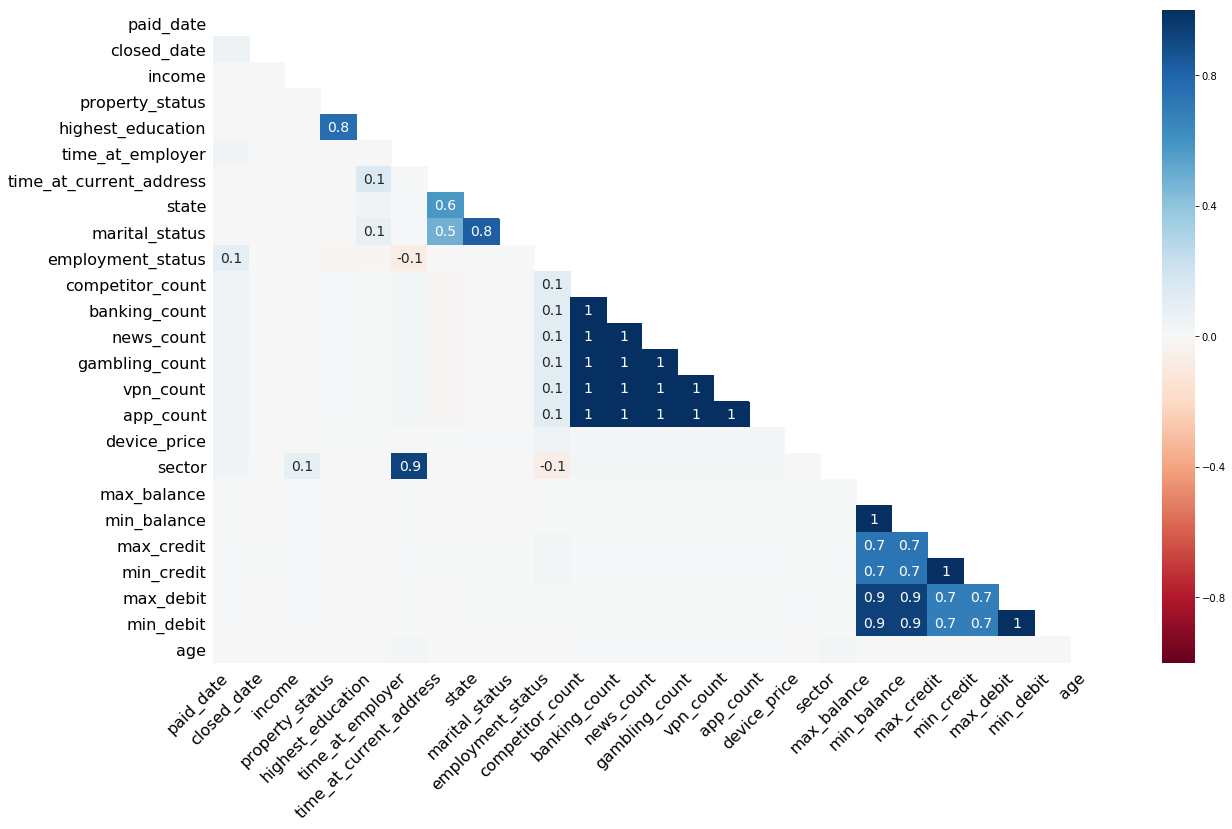
\includegraphics[width=0.95\textwidth]{images/nutility_correlation.png}
\caption{Nullity Correlation}
\label{fig:nullity}
\end{figure}

\vspace{10pt}

It can be seen from Figure \ref{fig:nullity} that no particular feature disparages the presence of another. However, the presence of certain features strongly correlates with the presence of other features. This is expected as no feature is sparsely populated. \\

 In data science projects, rows containing missing values are often removed from the dataset \parencite{MissingValues}. In the case of this project excluding all cases containing a missing value was not feasible as too few samples would have remained to train and test a valid model. This is because more than 50 percent of rows within the dataset contained at least one missing value. \\
 
 Table \ref{table:missing_row} displays the count of applicants, the cumulative count of applicants, and the percentage of total applicants that have the number of missing values shown in the first column of the table. Table \ref{table:missing_row} displays that 2.81\% of applicants have more than 10 missing values, while no loan applicant had more than 14 missing values. The total number of dependent variables used is 53.   
 
\vspace{10pt}

\begin{table}[H]
\begin{center}
\begin{tabular}{|c|c|c|c|} 
\hline
\multicolumn{1}{|c|}{Missing Values}
&\multicolumn{1}{|c|}{Count}
&\multicolumn{1}{|c|}{Cumulative Count}
&\multicolumn{1}{|c|}{Percentage of Total}\\
\hline
0 & 28,808 & 28,808  & 45.77  \\
\hline
1 & 6,276 & 35,084 & 55.75  \\
\hline
2 & 6,275 & 41,359 & 65.72 \\
\hline
3 & 1,495 & 42,854 & 68.09 \\
\hline
4 & 577 & 43,431 & 69.01 \\
\hline
5 & 97 & 43,528 & 69.16 \\
\hline
6 & 12,500 & 56,028 & 89.03 \\
\hline
7 & 3,516 & 59,544 & 94.61 \\
\hline
8 & 1,168 & 60,712 & 96.47 \\
\hline
9 & 376 & 61,088 & 97.07\\
\hline
10 & 75 & 61,163 & 97.19\\
\hline
11 & 21 & 61,184 & 97.22\\
\hline
12 & 1,046 & 62,230 & 98.88\\
\hline
13 & 623 & 62,853 & 99.87\\
\hline
14 & 81 & 62,935 & 100.00\\
\hline
\end{tabular}
\end{center}
\caption{Number of Missing Values by Observation/Applicant}
\label{table:missing_row}
\end{table}

Another common missing value imputation technique involves replacing missing values with the mean (continuous variables) or mode (categorical variables) of their respective variable. This is a successful technique if the variables are considered to be missing at random. In the case of this project missing values were consider to be missing not at random. This is due to the fact that the loanees manually filled certain variables during their loan applications. Loanees may have withheld or altered variables based on how they thought it would affect the outcome of their credit application \parencite{MissingValuesBos}. \\

There are many methods for imputing missing values where the values are missing not at random. The two methods explored were SVD (singular value decomposition) and k-nearest neighbours. \\

SVD involves calculating a matrix's mutually orthogonal eigenvectors. The most important eigenvectors are then linearly combined in order to best predict the missing values of the matrix. In the case of the dataset used in this project, each loan application would be considered as a matrix row and the predictor variables would be the respective columns. An issue with SVD imputation is that the predictions for missing values are calculated using the most important eigenvectors and not all eigenvectors. Therefore, in terms of this project, unusual loan cases would not be well represented by the leading eigenvectors and as a result their missing values may not be accurately filled. This lead to the KNN approach being used \parencite{MissingValuesStandford}. \\

The KNN approach involves filling the missing values of a particular row with the average value of the equivalent variable from the row's K "most similar" neighbours. Similarity can be calculated using various distance metrics, for example Euclidean, Minkowski, and Manhattan distances. Equation \ref{eq:eucidean} shows the Euclidean distance between points x and y. The distance is calculated by taking the square root of the sum of the squared differences between the respective variables of each point \parencite{EuclideanDist}. 

\vspace{10pt}

\begin{equation} \label{eq:eucidean}
d(x,y)=\sqrt{(x_{1}-y_{1})^{2} + (x_{2}-y_{2})^{2} + ... + (x_{n}-y_{n})^{2}}
\end{equation}

\vspace{10pt}

Before the KNN model was developed to replace the missing values in the dataset, each variable was normalised and scaled. This was done for both categorical and numeric variables. The methods used to do this are explained in sub-section 3.3.1.\\

After normalisation and scaling, the following steps were completed in order to fill missing values for each loan in the dataset using the KNN approach: 

\begin{enumerate}
    \item Set the number of nearest neighbours to be considered for each loan to 3 (arbitrary selection).
    \item Check if the loan had any missing values. If the loan did not have missing values move to the next loan, if it did then continue to the steps below. 
    \item Calculate the Euclidean distance between the loan under consideration and every other loan. 
    \item Identify the 3 closest loan applications based upon Euclidean distance. 
    \item Fill each missing value with the mean value of the respective variable taken from the loan's 3 nearest neighbours. 
\end{enumerate}

\subsection{Outlier Detection}

Outlier detection involves identifying observations that have features that do not conform to the typical patterns of the features of other observations \parencite{Outlier1}. In this project, outliers are detected using the isolation forest algorithm, which is an unsupervised extension of the decision tree algorithm. The isolation forest algorithm does not require distances or densities to be calculated between data points to identify outliers, which leads the algorithm to have a low computational cost \parencite{Outlier2}.  \\

The isolation forest algorithm involves training a decision tree - in a unsupervised manner - by recursively splitting a dataset until each observation becomes terminal node on the tree. This process is displayed in Figure \ref{fig:isolation}. We can see from the figure that the furthest right observation was isolated after only two splits. While, the highlighted observation towards the bottom of the diagram passed through 5 feature splits before becoming isolated. \\

The depth of each observation - the number of iterations before it is isolated  is recorded. This process is repeated multiple times and the average depth for each observation is calculated. Observations with a very small tree depth - relative to the depth of the other observations in the dataset - are considered to be anomalies \parencite{Outlier2}. \\

\vspace{10pt}

\begin{figure}[!htb]
\centering
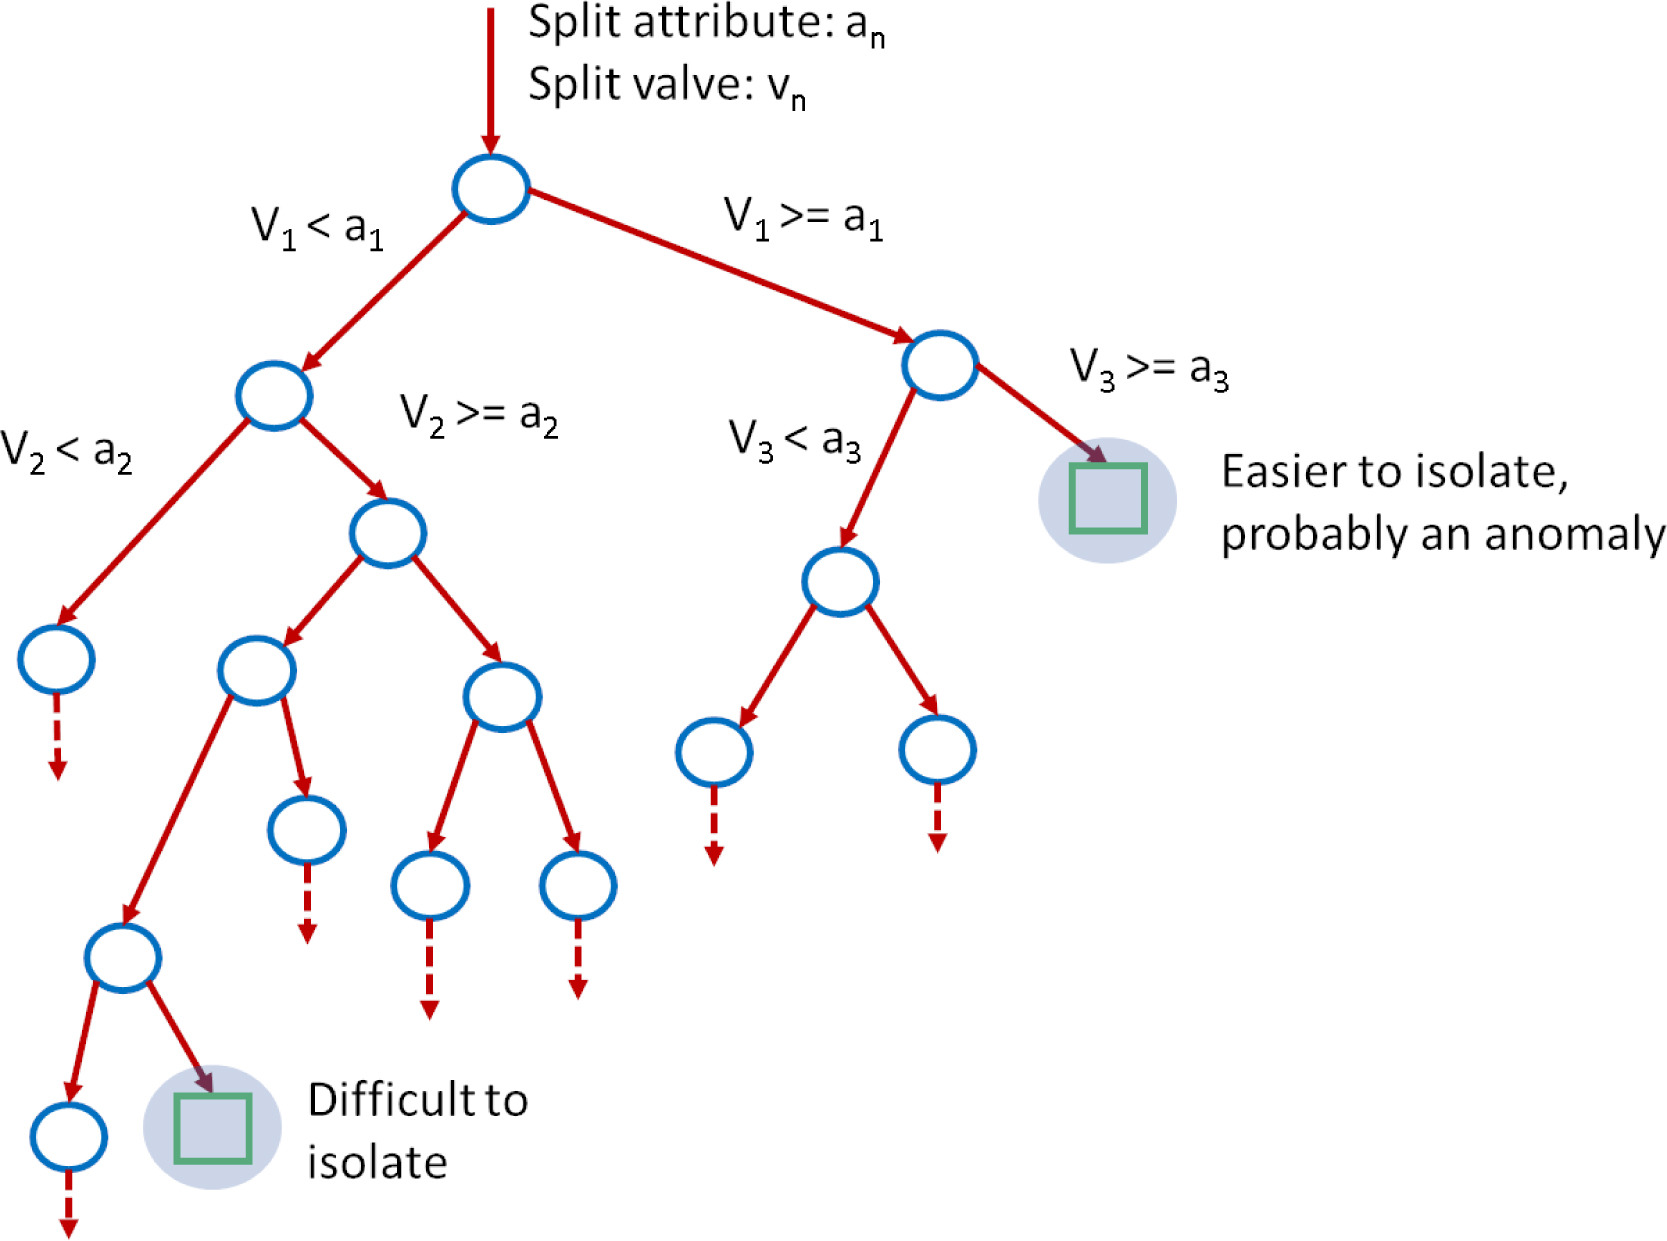
\includegraphics[width=0.9\textwidth]{images/isolation_tree.jpg}
\caption{Isolation Forest Principle}
\label{fig:isolation}
\parencite{Outlier1}
\end{figure}


In the case of this project, loan applicants with features that greatly vary from the features of the other applicants are identified by training an isolation model. Applicants that are deemed as outliers - 2,261 of the total 62,935 - by the isolation forest model are removed from the final dataset used to train the loan default prediction models. A default contamination ratio (suspected ratio of outliers in the dataset) of 0.1 is used to remove the outliers. The default ratio is used as no expected ratio could be attained. \\


\section{Summary of Data Extraction and Preprocessing}

Firstly, this chapter details the three data sources that are used in this project, namely sociodemographic data provided by the Nigerian micro-fiance company that provide the loan data, Nigerian credit bureau data, and the alternative features developed through web-scraping and regular expressions. Finally, the chapter details the pre-processing techniques used prior to modelling, which includes handling missing values, scaling variables, and handling outlier observations. \\

The next chapter details the 4 modelling techniques used throughout this project, namely logistic regression, random forest, XGBoost, and neural networks. Finally, the chapter discusses the feature selection methods used and how the various models are tested.  